\clearpage

\section{GraphRNN}\label{sec:graphrnn}\index{GraphRNN}

\begin{notebox}
\textbf{Paper: } \fullcite{you_graphrnn_2018}
\vspace{5pt}

\href{}{no reviews}
\hspace{1cm}
\href{https://github.com/snap-stanford/GraphRNN}{code}
\hspace{1cm}
\href{run:/home/magda/Dropbox/Zot/You et al_2018_GraphRNN.pdf}{Local pdf}
\vspace{3pt}

Read on 3/3/2022 for \iterm{Yoann}
\hfill Notes taken: 3/3/2022 \index{March 2022}
\end{notebox}

\begin{notebox}[colback=red!5]
\tldr Models the graph in \iterm{autoregressive} (\iterm{recurrent}) manner from its sequential representation. 
It is a hierarchical model with graph-level RNN to capture the state of the graph and edge-level generates edges for each new node included in the graph.
They use \iterm{breadth-first-search} (BFS) node ordering strategy through which they limit the number of possible node permutations in the sequence ordering.
\end{notebox}

\begin{notebox}[colback=yellow!5]
\textbf{Notes:} 
\begin{itemize}[nosep]
\item Very nice paper! 
\end{itemize}
\end{notebox}

They want to learn generative models for graphs. They put forward three main challenges:
\begin{itemize}[nosep]
\item large and variable output space - with $n$ nodes up to $n^2$ possible edges but may be variable
\item non-unique representation - up to $n!$ equivalent adjacency matrices with different node ordering (graph matching is $O(n^4)$)
\item complex structural dependencies - edges are not independent from one another
\end{itemize}

\begin{wrapfigure}{r}{0.5\textwidth}
\centering
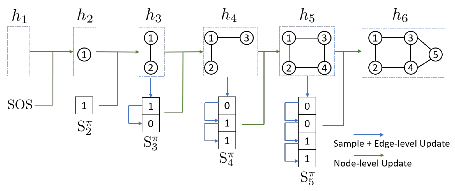
\includegraphics[width=0.5\textwidth]{graphrnn_Figure1.png}
\caption{Hierarchical model with graph-level RNN and state vectors $h_i$ and edge-level RNN predicting the adjacency vector $S_i^\pi$ that serves as input to the next graph-level step.}
\end{wrapfigure}
For graph $G=(V, E)$ we have a set $\Pi$ of $n!$ possible permutations $\pi$ of the nodes $V$ in the adjacency matrix $A^\pi \in \mR^{n \times n}$.
What they should learn is the $p_\theta(G)$ over graphs from training set generated from the true $p(G)$. 
They assume that the node ordering in the training set is random and uniform with $p(\pi) = \frac{1}{n!}, \ \forall \pi \in \Pi$.

They propose to model the graphs as sequences (allows for varying size) and use BFS to generate the sequences from the graph.
This should reduce the complexity of learning over all possible sequences. 
They rely on RNN where the main idea is to decompose the graph generation into two process.
The first generates a sequence of nodes (graph-level RNN) and the second generates the edges between each new node and the existing ones (edge-level RNN). 
(
They assume a mapping from graph to sequences (under ordering $\pi$) $S^\pi = f_s(G, \pi) = (S_1\pi, \ldots, \S_n^\pi)$, where each $S_i\pi \in \{0, 1\}^{i-1}$ is an adjacency vector with edges between node $\pi(v_i)$ and all nodes already in the graph $\pi(v_j), \ j<i$.
The sequence determines a unique graph through mapping $G = f_G(S^\pi)$.
However, instead of learning $p(G)$ they sample $\pi$  and learn $p(S^\pi)$ autoregressively.
They can sample $G$ by sampling $S^\pi$ and mapping it to the graph $G = f_G(S^\pi)$ with
$p(G) = \sum_{S^\pi} p(G, S^\pi) = \sum_{S^\pi} p(S^\pi) \mathbb{I}[f_G(S^\pi) = G]$.

They decompose the sequence distributions $p(S^\pi) = \Pi_{i=1}^{n+1} p(S^\pi_i |  S^\pi_{<i})$ and use an RNN with state-transision and output functions
\begin{align*}
h_i & = f_{trans}(h_{i-1}, S^\pi_{i-1}), \\
\theta_i & = f_{out}(h_i) \enspace, 
\end{align*}
where $S^\pi_{i-1}$ is the adjacency vector so far, $h_{i-1}$ is the state of the graph so far and $\theta_i$ specifies the binary vectors distribution of the next node's adjacency vector $S^\pi_{i} \sim p_{\theta_i}(S^\pi_i |  S^\pi_{<i})$.

They propose two variants: simple variant where $p_{\theta_i}(S^\pi_i |  S^\pi_{<i})$ is a multivariate Bernoulli; and sequence dependent Bernoulli, where $p_{\theta_i}(S^\pi_i |  S^\pi_{<i}) = \Pi_{j=1}^{i-1}p(S^\pi_{i, j} |  S^\pi_{i, <j}, S^\pi_{<i})$.

They argue strongly in favor of BFS to determine the node ordering.
They claim that in this way, they do not need to train over all possible node permutations but instead only over all the BFS orderings which are fewer as multiple orderings map to the same BFS. \note{I need fresh brain.}

\textbf{Experiments:} They introduce new experimental benchmarks - \iterm{community graphs} and \iterm{ego networks} dataset.
For evaluation they use \iterm{Maximum Mean Discrepancy} \iterm{MMD} over graph statistic distributions.
It works nicely.



